\section{问题三求解与分析}
\label{sec:q3}
\subsection{问题的描述与分析}
第三问保留第二问的核心级 Task、子图划分、核心归属与核内顺序，并在各核的读入路径前加入容量为 $1048576$ B 的共享只读 L2。缓存改变的是一部分 $\mathrm{COPY\_IN}$ 的服务路径，不改变计算图的依赖、写出要求或方案变量。若读入命中，数据经 L2 带宽池服务；未命中时仍经 DDR，并在完成后尝试填充。由此，哪一次请求能命中取决于全局读入发射、完成与淘汰的交错，而不仅取决于方案包含多少重复张量。

图~\ref{fig:q3_overview} 展示本问的分析与求解流程：以第二问完整方案空间为基础，记录真实缓存事件，从观察到的重复未命中或淘汰窗口提出合法核内顺序候选，再用完整执行评价决定是否接受。实验分为三种口径：100 图的第三问主结果，同一第三问方案有无 L2 的配对结果，以及六张定向图在固定方案下的容量、带宽格点。三者回答的问题不同，不能互相代替。
\begin{figure}[htbp]
\centering
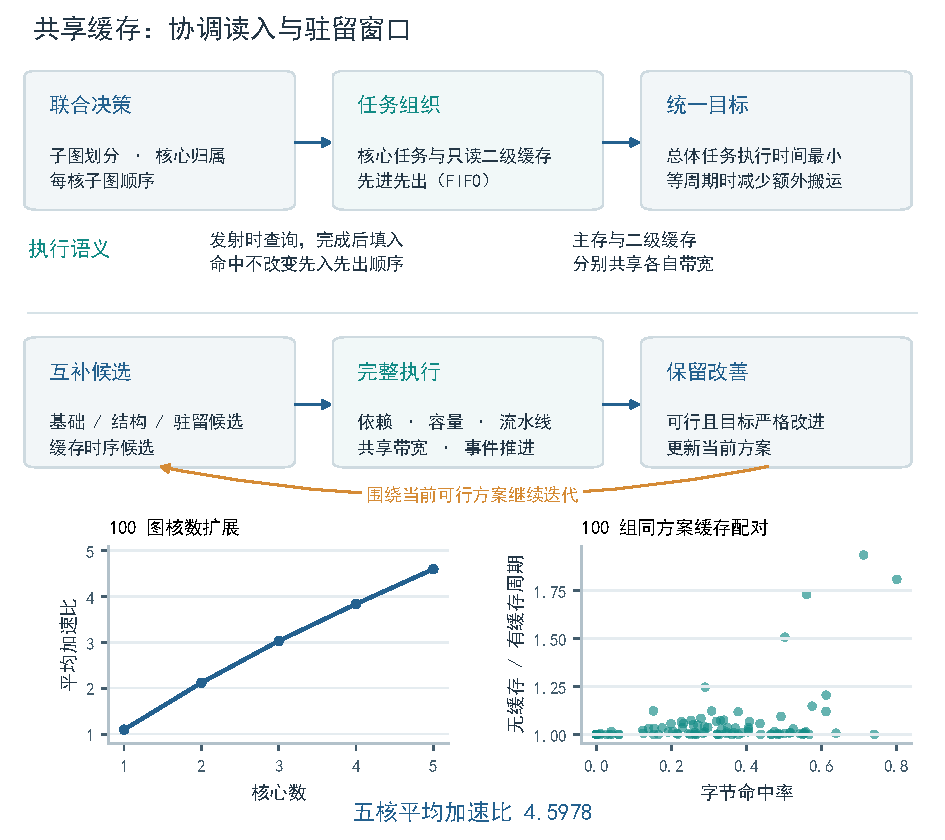
\includegraphics[width=\textwidth]{../求解/问题三/图片/q3_overview.pdf}
\caption{问题三的联合建模与迭代改进框架}\label{fig:q3_overview}
\end{figure}


\subsection{共享只读 L2 的事件模型}
\subsubsection{发射查询、完成填充与 FIFO 顺序}
记全局缓存状态 $\mathcal Q(\tau)$ 为按成功填入先后排列的逻辑张量标识队列，其容量用队列内张量字节之和计。对张量 $t$ 的一次读入请求 $r$，在其实际发射时刻 $s_r$ 查询 $\mathcal Q(s_r)$。若命中，则读入由 L2 池服务，且该次命中不将 $t$ 移至队尾；若未命中，则请求由 DDR 池服务。未命中读的完成时刻 $f_r$ 才触发填充尝试，需为 $t$ 腾出空间时从队首依次淘汰最早填入的对象。尺寸超过容量的张量不驻留。图~\ref{fig:q3_fifo} 按事件轴表示这一先查询、后填充的过程。
\begin{figure}[htbp]\centering
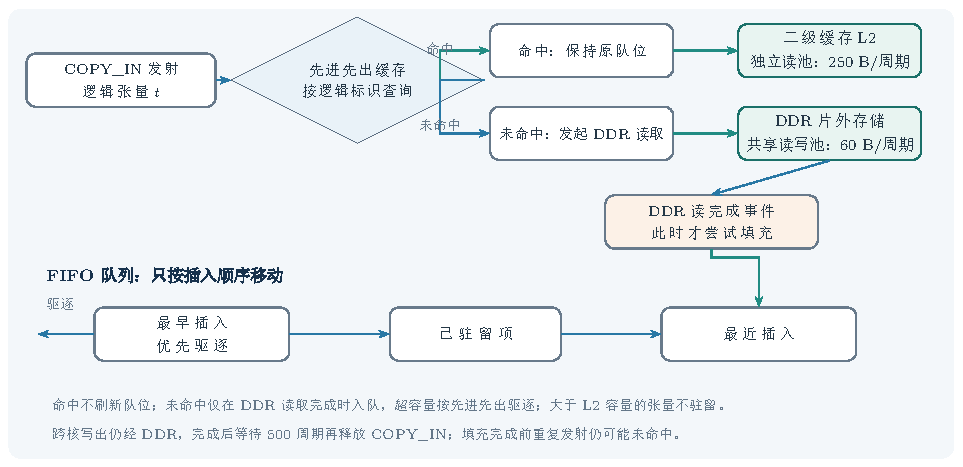
\includegraphics[width=.96\textwidth]{../求解/问题三/图片/q3_fifo.pdf}
\caption{FIFO 读入查询、完成填充与淘汰事件}\label{fig:q3_fifo}
\end{figure}

这一规则尤其影响并发读入。若两核在 $t$ 首次 DDR 读尚未完成时先后发射对 $t$ 的请求，二者查询时 $t\notin\mathcal Q$，可以同时未命中；不能把第二次发射误当作第一次读的必然命中。另一方面，已命中的张量即使频繁被读取，也不会因命中刷新 FIFO 位置，后续插入仍可能将其淘汰。因此，按“最近一次使用距今多远”预测命中并不符合这里的规则。已有缓存感知 DAG 调度研究讨论了节点亲和性与延迟执行\cite{A40}，其 LRU 更新和周期性作业假设与本题的完成填充、命中不更新的 FIFO 不同；本文仅采用“执行时序会改变复用机会”的一般动机，命中由本题事件定义计算。

一份真实执行轨迹说明上述时间差。某张量在周期 $0$ 的读入发射时未命中，于周期 $345$ 填入；其他对象连续填入后，它在周期 $5254$ 被淘汰，并在周期 $10823$ 再次读入时未命中。同一轨迹中另有张量在填入后发生命中。这个例子表明，逻辑上存在复用并不等于相关读入处于缓存驻留窗口内；候选应围绕具体发射、填充和淘汰事件调整顺序，而不是仅统计重复使用次数。

\subsubsection{两个共享服务池与计量口径}
设时刻 $\tau$ 在途 DDR 和 L2 读请求集合分别为 $\mathcal A_D(\tau)$ 与 $\mathcal A_L(\tau)$。两池分别以 $60$ B/周期和 $250$ B/周期的总带宽服务，并按各自在途请求数共享；在事件集合不变的区间，某请求以独占服务周期表示的剩余量满足
\begin{equation}
 w_j(\tau+\Delta)=
 \max\!\left\{0,w_j(\tau)-\frac{\Delta}{|\mathcal A_h(\tau)|}\right\},
 \quad j\in\mathcal A_h(\tau),\quad h\in\{D,L\}.
 \label{eq:q3_two_pools}
\end{equation}
这里两种 $w_j$ 分别按本池带宽换算，不能把 $60$ 与 $250$ 简单相加为单条读请求的带宽。DDR 写出和未命中读仍与其他 DDR 请求争用；命中读虽不经 DDR，仍占 L2 池及对应读入流水线，并可能受前驱、缓冲容量和核心内部顺序约束。一次命中降低的是这次读的 DDR 服务需求，不自动减少总体完成周期。

设 $B_i^{\rm hit}$ 与 $B_i^{\rm miss}$ 为某执行中 \texttt{COPY\_IN} 经 L2 命中和未命中的字节，定义按字节计的命中率
\begin{equation}
 H_i=\frac{B_i^{\rm hit}}{B_i^{\rm hit}+B_i^{\rm miss}}.
 \label{eq:q3_hit}
\end{equation}
当分母非零时，$H_i$ 描述读入服务路径的比例，而非周期收益比例。第~\ref{sec:q1} 节的 $D_3(x)$ 是额外 COPY 字节口径；即使命中，它对应的逻辑读入操作仍可能计入 COPY，故 $D_3$ 既不等于实际 DDR 字节，也不能从 $H_i$ 单独推出。最终周期还由计算关键链、写出、两池并发以及填充造成的 FIFO 变化共同决定。

\subsection{缓存时序候选与统一接受规则}
\subsubsection{合法顺序邻域}
第三问沿用基础、结构和驻留候选，并增设由已评价缓存轨迹驱动的顺序候选。设当前方案为 $x=(\mathcal P,a,\boldsymbol\pi)$，此来源产生的 $x'=(\mathcal P,a,\boldsymbol\pi')$ 保持算子到子图的划分及子图到核心的归属，只在一个或两个核心的 $\pi_k$ 中移动完整子图。于是原始算子覆盖、每个算子的核心归属与跨核边集合保持不变；但局部先后、读入发射时刻、Spill、FIFO 队列和完成时刻都可能变化。该不变量并不保证无环，候选仍须检查与跨核依赖相容的核序，再作完整执行评价。

从实际未命中记录中，可辨别读入发射时尚有相同张量的在途填充、或上一次缓存副本已被淘汰两类窗口。第一类候选试着将消费者子图后移，或把产生首次有效填充的读者子图前移，让后续发射有机会落在填充之后。第二类候选试着把消费者前移，或把引发实际淘汰的填入者后移，让复用落在淘汰之前。还可联合不同核心上的两次局部移动，并按相邻子图的计算工作量估计需要跨过的时间窗口。移动距离仅是提出候选的启发，不预言新执行必然命中；移动后所有请求的交错会重新生成。候选在来源内去重，经过结构下界和完整执行，才按 $(C_3,D_3)$ 的字典序与当前方案比较。

图~\ref{fig:q3_fifo} 中的填充与淘汰窗口可解释为何仅做“把相同张量的消费者相邻排列”还不够：执行层面决定 FIFO 顺序的是成功填入时刻，而不是方案中静态的子图距离。候选来源仍按第~\ref{sec:q1} 节的近期实测收益、运行成本和访问间隔分配机会。测量反馈用于有限搜索资源安排的思想与程序自动调优工作相通\cite{A12}；这里没有训练其成本模型，也不据来源选择指数声称概率最优。所有来源共享同一当前可行方案，结构或驻留候选被接受后，缓存事件候选会围绕新的执行轨迹重新提出。

\subsubsection{同方案配对的识别量}
令 $x_{i,3,n}$ 为图 $i$、$n$ 核下第三问选出的完整方案。将\emph{同一个方案}分别置于有 L2 和无 L2 的执行环境，定义
\begin{equation}
 R^{\rm L2}_{i,n}=
 \frac{C_2(x_{i,3,n})}{C_3(x_{i,3,n})}.
 \label{eq:q3_pair}
\end{equation}
两次执行保持 $\mathcal P,a,\boldsymbol\pi$ 一致，改变的是缓存规则；若同一配置的配对响应完整且可行，式~\eqref{eq:q3_pair} 才可解释为该固定方案的缓存影响。分子不能使用第二问单独寻优得到的 $C_2(x_{i,2,n})$，因为那同时改变了方案。即使 $R^{\rm L2}_{i,n}>1$，它也不代表所有可能方案的缓存平均效应：样本方案是第三问搜索选择的，且缓存可改变哪些方案被偏好。

\subsection{主实验与定向参数研究}
\subsubsection{核数扩展、独立优化与同方案对照}
第三问仍用式~\eqref{eq:speedup} 的逐图算术平均。表~\ref{tab:q3_mean} 与图~\ref{fig:q3_mean} 给出一至五核主结果，平均加速比分别为 $1.1008$、$2.1222$、$3.0320$、$3.8376$、$4.5978$，五核中位数为 $4.8565$。一核结果可以高于 1，因为原始单核参考没有按第三问的方案和缓存条件重新优化；多核结果也包含重新分组与顺序的影响。图中另以相同第三问方案的无 L2 响应构成参考曲线，其含义由式~\eqref{eq:q3_pair} 确定。
% 由求解/规范化数据/combined/means.csv 生成；逐图加速比的算术平均。
\begin{table}[htbp]
\centering\small
\setlength{\tabcolsep}{5pt}
\begin{tabular}{rrrrrr}
\toprule
核心数 & 样本数 & 平均加速比 & 中位加速比 & 最小加速比 & 最大加速比 \\
\midrule
1 & 100 & 1.1008 & 1.0427 & 0.9969 & 2.0540 \\
2 & 100 & 2.1222 & 2.0271 & 1.5225 & 3.6533 \\
3 & 100 & 3.0320 & 3.0182 & 1.7667 & 5.4726 \\
4 & 100 & 3.8376 & 3.9656 & 1.9853 & 7.0949 \\
5 & 100 & 4.5978 & 4.8565 & 2.0717 & 8.7768 \\
\bottomrule
\end{tabular}
\caption{问题三各核数逐图加速比统计}\label{tab:q3_mean}
\end{table}

\begin{figure}[htbp]\centering
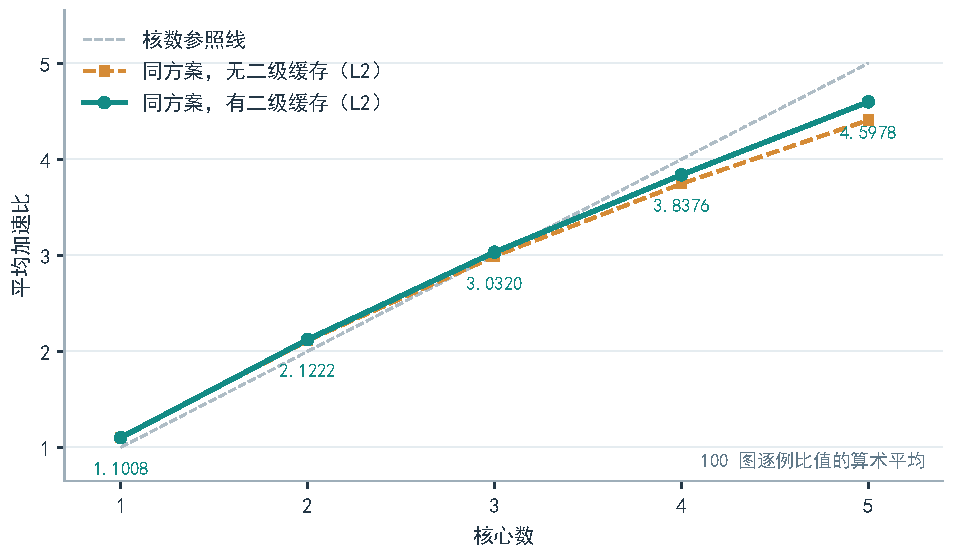
\includegraphics[width=.91\textwidth]{../求解/问题三/图片/q3_mean.pdf}
\caption{第三问各核数主结果及同方案无 L2 参考}\label{fig:q3_mean}
\end{figure}

若改用两问各自选出的五核方案相较，第三问在 100 图中有 66 图周期短于第二问、18 图相等、16 图更长。这个对照描述两问独立搜索的最终表现，不属于固定方案缓存试验。第三问五核额外 COPY 字节均值为 $8293721.4$ B，中位数为 $1484117$ B；这些数可以与第二问的口径直接比较，却不能视为实际 DDR 访问量。缓存改变请求路径和候选偏好后，逻辑 COPY、自动换出和服务资源都会变化。

同方案配对覆盖 100 图的全部五种核数，共 500 组。各核数样本量、平均和中位周期比列于表~\ref{tab:q3_pairs}，经验分布见图~\ref{fig:q3_pairs}。五核平均周期比为 $1.0558$，中位数为 $1.0077$；77 图的周期缩短，23 图相等。曲线在 1 附近的集中程度表明许多方案虽有缓存，关键完成时刻并未明显移动；右侧尾部显示少数图的固定方案得到更大收益。
% 由同一方案的有/无 L2 双响应计算；比值为无 L2 周期/有 L2 周期。
\begin{table}[htbp]
\centering\small
\setlength{\tabcolsep}{4pt}
\resizebox{160mm}{!}{%
\begin{tabular}{rrrrrrrr}
\toprule
核心数 & 配对数 & 平均周期比 & 中位周期比 & 改善 & 相同 & 退化 & 平均字节命中率 \\
\midrule
1 & 100 & 1.0003 & 1.0000 & 28 & 72 & 0 & 0.0599 \\
2 & 100 & 1.0047 & 1.0001 & 58 & 42 & 0 & 0.1757 \\
3 & 100 & 1.0156 & 1.0009 & 66 & 34 & 0 & 0.2342 \\
4 & 100 & 1.0304 & 1.0018 & 71 & 28 & 1 & 0.2470 \\
5 & 100 & 1.0558 & 1.0077 & 77 & 23 & 0 & 0.3017 \\
\bottomrule
\end{tabular}
}%
\caption{第三问同一方案有无 L2 的周期配对统计}\label{tab:q3_pairs}
\end{table}

\begin{figure}[htbp]\centering
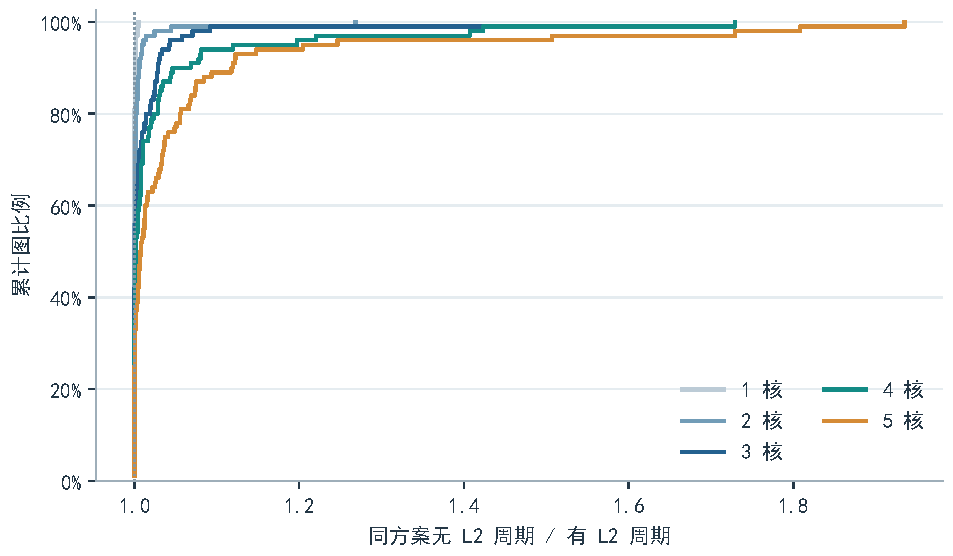
\includegraphics[width=.92\textwidth]{../求解/问题三/图片/q3_pairs.pdf}
\caption{各核数同方案缓存周期比的经验分布}\label{fig:q3_pairs}
\end{figure}

图~\ref{fig:q3_hit_gain} 对照逐例命中字节率与式~\eqref{eq:q3_pair}。二者可能同向变化，但关系不应被强制写成直线：命中若落在非关键请求上，可能不改变 总体任务执行时间；低命中率也可能恰好覆盖关键链上的少量大请求。图的点位以真实配对响应计算，适宜显示异质性，而不等同于控制了计算链、写出与两个带宽池后的因果估计。第三问主结果的全局下界与当前五核周期给出的相对差距上界逐图平均为 $0.2248$；其中 6 图在 $1\%$ 以内。该界沿用计算路径、Pipe 负载与可证明必要流量的松弛，不能把缓存未命中次数直接加进全局下界。
\begin{figure}[htbp]\centering
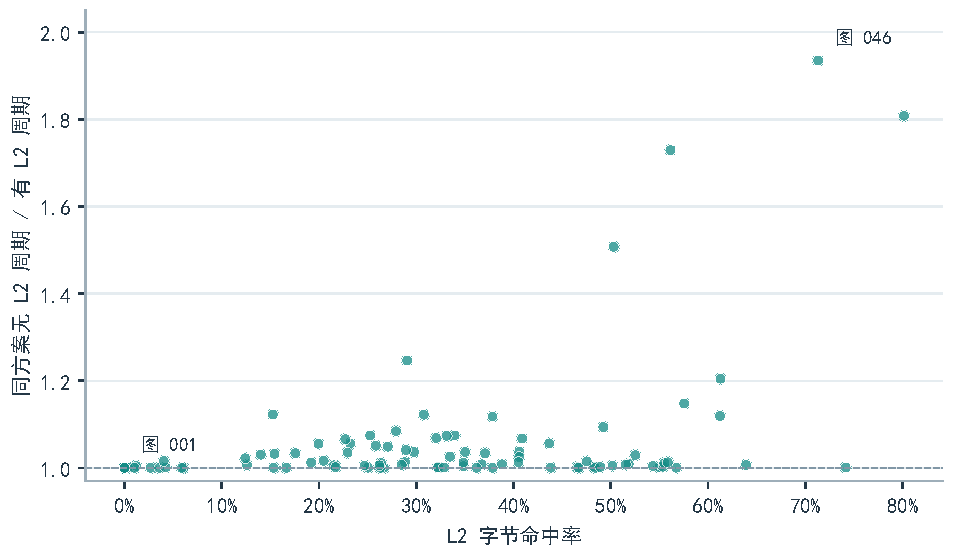
\includegraphics[width=.92\textwidth]{../求解/问题三/图片/q3_hit_gain.pdf}
\caption{字节命中率与同方案缓存周期比}\label{fig:q3_hit_gain}
\end{figure}

\subsubsection{固定方案的容量—带宽响应面}
为观察参数敏感性，从主实验中定向选取六张图，每图固定一份五核完整方案，分别在 L2 容量 $262144$、$1048576$、$4194304$ B，与 L2 带宽 $60$、$250$、$500$ B/周期的九个组合下执行。图~\ref{fig:q3_parameters} 展示共 54 个固定方案格点的真实周期；其中各图的默认配置格沿用对应主实验响应。由于一张图的九格使用同一划分、归核和顺序，格内差异可归于该方案在参数变化下的执行映射，而非方案搜索变化。样本是按机制价值定向选取的六图，不能把格点平均解释为 100 图总体的硬件敏感性。
\begin{figure}[htbp]\centering
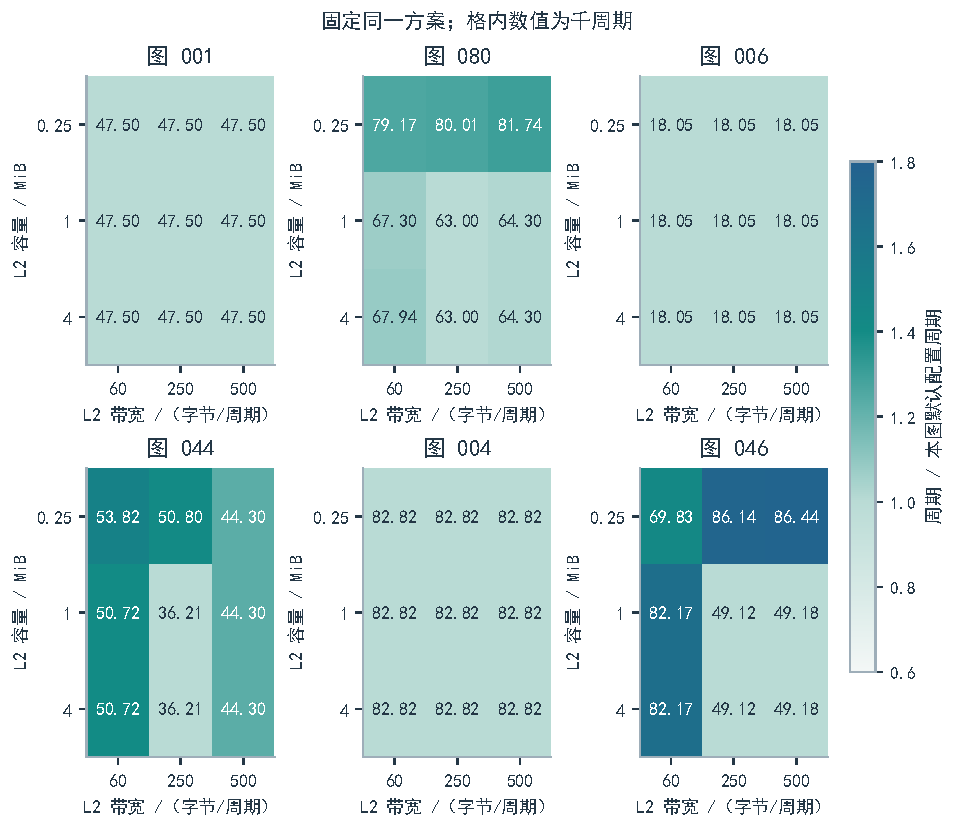
\includegraphics[width=.96\textwidth]{../求解/问题三/图片/q3_parameters.pdf}
\caption{六图固定方案的 L2 容量与带宽周期响应}\label{fig:q3_parameters}
\end{figure}

图80在带宽固定为 $250$ B/周期时，容量从 $262144$ B 增至 $1048576$ B，周期从 $80014$ 降至 $63001$，字节命中率从 $0.1827$ 升至 $0.5031$。图1的九个格点均为 $47502$ 周期且零命中，表明提高缓存容量或 L2 带宽只有在相应读入真正利用缓存并影响完成路径时才可能奏效。另有每图两个边端参数配置允许在有限预算内重新适配方案，共 12 个观察值；这类结果把参数变化和方案变化合在一起，已与固定方案九宫格分开，不用于估计单独的容量或带宽效应。

由事件、配对与参数格可见，第三问的关键不是抽象地提高重复读取比例，而是使关键请求的发射落在有效 FIFO 驻留窗口内，并避免把新争用转移到 L2 池或读入 Pipe。统一的完整方案评价给出可行周期，同方案配对识别固定方案的缓存影响，定向格点揭示响应的图依赖性；三者共同构成对缓存机制的检验。

\subsection{缓存驻留窗口的推导与逐事件分析}
\subsubsection{先入先出驻留窗口}
缓存时序候选需要判断一次顺序移动究竟试图跨过哪个事件。为此，考察张量 $t$ 在时刻 $f_t$ 成功填入后的这一段驻留期。设其大小为 $b_t\le B_{\mathrm{L2}}$，定义 $A_t(\tau)$ 为 $(f_t,\tau]$ 内在它之后成功新填入队列的对象字节总和。已经在队列中的对象被再次查询或填充时不重复计入；不驻留的超大对象也不计入。这里的“新填入”取自执行事件序列，因此包含不同核心发起请求的全局交错。

\textbf{命题4：}在只按先进先出规则因容量不足淘汰、命中不刷新位置的条件下，张量 $t$ 的首次淘汰发生于第一个使 $b_t+A_t(\tau)>B_{\mathrm{L2}}$ 的新填入事件。在此前的查询时刻，$t$ 仍驻留于缓存。

\textbf{证明：}张量 $t$ 插入时，原队列中的对象均排在它之前。新对象始终排在其后。只要 $t$ 尚未淘汰，排在它之后的对象也不会先被淘汰；故这些对象的实际总大小正是 $A_t(\tau)$。若 $b_t+A_t(\tau)\le B_{\mathrm{L2}}$，即使空间不足，也只需淘汰足够多的旧前缀，仍能容纳 $t$ 及其后的全部对象，无需淘汰 $t$。若首次超过容量，旧前缀即便已全部移除也不足以腾出空间；先进先出规则随后必定淘汰 $t$。由事件次序归纳即得结论。证毕。

因此，若一次消费者读入发射于 $s_t$，要利用这段驻留期，需要该发射在完成填充之后、首次淘汰之前，即落入相应事件序上的区间。设首次淘汰时刻为 $e_t$，对无同刻歧义的事件有
\begin{equation}
 f_t\le s_t<e_t.
 \label{eq:cachewindow}
\end{equation}
若填充、淘汰或查询具有相同周期，还须使用执行器在该周期内的实际事件顺序判断端点；周期相等并不等价于队列状态相同。缓存命中对队列顺序没有影响，所以窗口不能仅由“上一次访问距今多久”描述，而应由填充后进入缓存的字节量及其先后次序描述。这也是缓存时序候选分别尝试调整首次填充、消费者与淘汰者的依据。

式~\eqref{eq:cachewindow} 是固定事件序列的性质。移动子图会改变计算完成、请求发射与带宽共享，进而同时改变 $f_t$、$e_t$ 和 $s_t$。实际方法据原轨迹提出移动方向，再重建整个执行过程；新方案中的驻留窗口随新轨迹重新确定。

\subsubsection{图80的填充、命中与淘汰}
取参数研究中图80的五核固定方案，L2 容量为 $262144$ B，带宽为 $60$ B/周期。图~\ref{fig:q3_trace} 展示原执行中两个张量的事件及开始阶段的读入流水线。为使图中文字易读，将原标识 $1000000001$ 与 $1000000187$ 分别简记为张量甲和张量乙；其大小分别为 $4096$ B 与 $8192$ B。
\begin{figure}[htbp]\centering
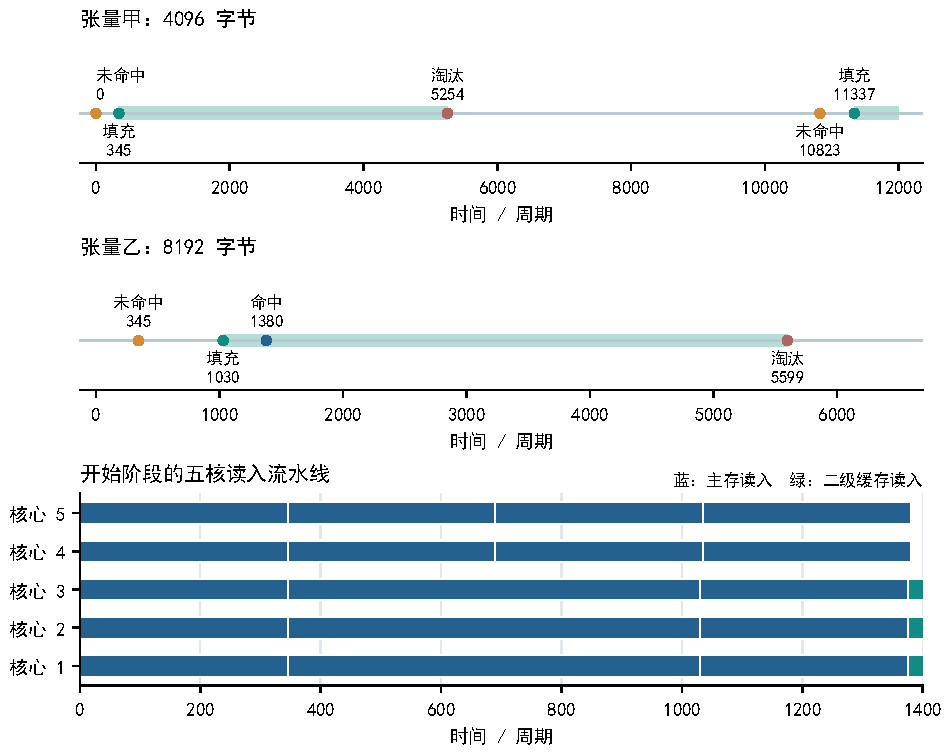
\includegraphics[width=\textwidth]{../求解/问题三/图片/q3_trace.pdf}
\caption{图80的缓存驻留窗口与多核读入轨迹}\label{fig:q3_trace}
\end{figure}

张量甲在周期0的读取未命中，读入于周期345完成后进入缓存。周期5254的一次新填入将它淘汰；当另一核心在周期10823再次读入甲时，访问已落在这段驻留窗口之外，因此再次未命中。甲在周期11337重新填入，于周期15878再次被淘汰；周期21536的下一次读取仍未命中。原图中存在重复消费，但这些消费跨越了有效驻留期，重复本身并未转化为命中。

张量乙在周期345查询时未命中，于周期1030填充；周期1380的查询发生在其驻留期内，因而命中。此命中没有将乙移至队尾，周期5599它仍被后续填入淘汰。两个张量形成直接对照：甲的后续读入晚于淘汰，乙的一次后续读入早于淘汰。顺序候选的目标由此可具体表述为提前某个消费者、推迟造成淘汰的填入者，或提前首次有效填充，而不必将所有重复消费者强制合并到同一子图。

图中最早的五个读请求均在周期0发射、周期345完成，显示共享 DDR 上的并发服务。对甲的 $4096$ B 请求，按每请求独占服务周期向上取整得到 $\lceil4096/60\rceil=69$ 周期；在这五个请求同时在途的区间，共享服务使其完成周期与 $5\times69=345$ 一致。随后各核读入的完成时刻分化，表明请求工作量和在途集合不断变化，不能用固定的五倍因子描述整个执行。

\subsubsection{容量与带宽的非线性作用}
参数格还显示了一个仅看带宽数值容易遗漏的现象：图80在 $262144$ B 容量下，L2 带宽从 $60$ 增至 $250$ 和 $500$ B/周期，周期依次为 $79170$、$80014$ 和 $81744$；图44在 $1048576$ B 容量下，对应周期为 $50723$、$36208$ 和 $44299$。这些值均来自每张图同一完整方案。提高缓存读带宽会提前部分操作，从而改变后续读的发射、完成填充和先进先出队列；在执行状态随之改变的条件下，局部服务变快并不强制整体周期单调下降。

同方案配对中也存在很小的周期反例：图79四核的有 L2 与无 L2 周期分别为 $7614798$ 与 $7614729$，相差69周期，二者额外 COPY 均为 $30445568$ B；该方案字节命中率约为 $0.2804$。相反，图46五核同方案的有 L2 与无 L2 周期分别为 $49119$ 与 $95050$，周期比为 $1.9351$，字节命中率约为 $0.7132$。这些逐例数值与命题4共同说明：缓存评价应追踪关键请求的实际驻留窗口和共享服务，字节命中率适合作为机制指标，总体任务执行时间仍是最终判据。

